
%-------------------------------------------------------------------------%
\section{The Standard Model}


\begin{table}[htbp]
    \centering
    \begin{tabular}{||c|c|c|c||}
    \hline
    & Gen1 & Gen2 & Gen3 \\
    \hline
    \multirow{2}{1.2cm}{quarks} & $u$ & $c$ & $t$ \\
     & $d$ & $s$ & $b$ \\
    \hline
    \multirow{2}{1.2cm}{leptons} & $e$ & $\mu$ & $\tau$ \\
     & $\nu_e$ & $\nu_\mu$ & $\nu_\tau$ \\
    \hline
    \end{tabular}
    \caption{The three generation of fermionic matter in the Standard Model.}
    \label{tab:SMFerm}
\end{table}



\begin{table}[htbp]
    \centering
    \begin{tabular}{||c|c||}
    \hline
       Gauge Bosons  & Scalar Bosons \\
     \hline
       $g$, $\gamma$, $Z$, $W^\pm$ & $H^0$ \\
     \hline
    \end{tabular}
    \caption{Force carriers (bosons) in the Standard Model.}
    \label{tab:SMBos}
\end{table}




\begin{figure}[htbp]
    \centering
    \begin{subfigure}{0.45\linewidth}
        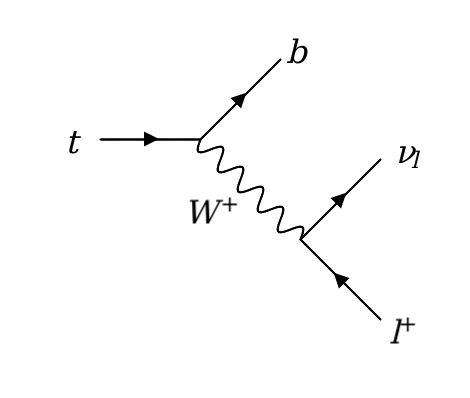
\includegraphics[width=\linewidth]{t_decay.png}
        \caption{top decay}
        \label{fig:top}
    \end{subfigure}
    \begin{subfigure}{0.45\linewidth}
        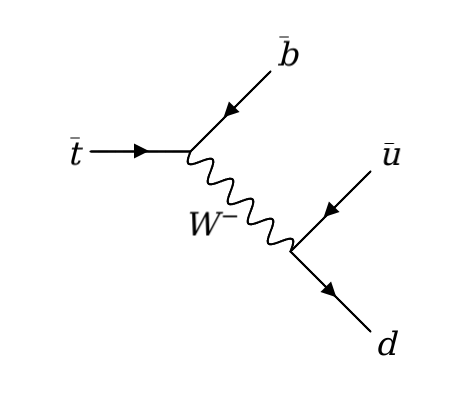
\includegraphics[width=\linewidth]{antt_decay.png}
        \caption{anti-top decay}
        \label{fig:anttop}
    \end{subfigure}
    \caption{Feynman diagrams of (anti-)top decays (examples).}
    \label{fig:decayDiag}
\end{figure}

%-------------------------------------------------------------------------%
\section{The Minimal Supersymmetric Standard Model (MSSM)}


\begin{table}[htbp]
    \centering
    \begin{tabular}{||c|c|c|c||}
    \hline
    & Gen1 & Gen2 & Gen3 \\
    \hline
    & \\[-2.7ex]
    \multirow{2}{1.4cm}{squarks} & $\Tilde{u}$ & $\Tilde{c}$ & \small$\Tilde{t}$ \\
     & $\Tilde{d}$ & $\Tilde{s}$ & $\Tilde{b}$ \\
    \hline
    
    \multirow{2}{1.4cm}{sleptons} & $\Tilde{e}$ & $\Tilde{\mu}$ & $\Tilde{\tau}$ \\
     & $\Tilde{\nu_e}$ & $\Tilde{\nu_\mu}$ & $\Tilde{\nu_\tau}$ \\
    \hline
    \end{tabular}
    \caption{The super-partners of the quarks and leptons in the SM.}
    \label{tab:SUSYspart}
\end{table}

\begin{table}[htbp]
    \centering
    \begin{tabular}{||c|c||}
    \hline 
       Gauginos  & Higgsinos \\
       \hline
        & \\[-2.5ex]
      $\Tilde{g}$, $\Tilde{\gamma}$, $\Tilde{B}$, $\Tilde{W}$ & $\Tilde{H}$ \\
     \hline
    \end{tabular}
    \caption{The super-partners of the Force carriers in the SM.}
    \label{tab:SUSYinos}
\end{table}


\begin{align}
     Q\ket{\text{Fermionic}} = \ket{\text{Bosonic}} 
     \label{eq:states1}
     \\
     Q\ket{\text{Bosonic}} = \ket{\text{Fermionic}}
     \label{eq:states2}
\end{align}




\begin{equation}
    P_R=(-1)^{3(B-L)+2s}
    \label{eq:MPrec}
\end{equation}

